\documentclass[multi=tikzpicture,border=8pt]{standalone}
\usepackage[UTF8]{ctex}
\usepackage{amsmath,amssymb,tikz}
\usetikzlibrary{arrows.meta,calc}
\definecolor{blue}{HTML}{17365D}
\definecolor{red}{HTML}{AC3931}
\tikzset{every node/.style={font=\small},arrow/.style={-{Stealth[length=2.8mm]},thick},dim/.style={|<->|,thin},box/.style={draw,rounded corners,align=center,minimum width=2.5cm,minimum height=.8cm}}
\begin{document}
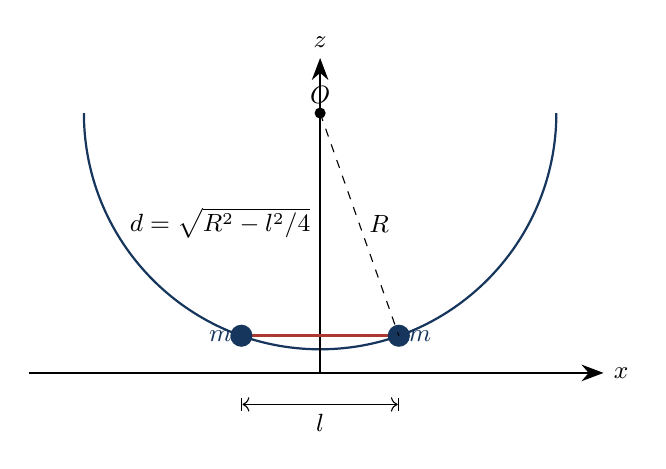
\begin{tikzpicture}

\draw[blue,thick](-3,0)arc(180:360:3);\fill(0,0)circle(2pt)node[above]{$O$};\draw[arrow](-3.7,-3.3)--(3.6,-3.3)node[right]{$x$};\draw[arrow](0,-3.3)--(0,.7)node[above]{$z$};
\draw[very thick,red](-1,-2.828)--(1,-2.828);\fill[blue](-1,-2.828)circle(4pt)node[left]{$m$};\fill[blue](1,-2.828)circle(4pt)node[right]{$m$};\draw[dashed](0,0)--(1,-2.828)node[midway,right]{$R$};\draw[dim](-1,-3.7)--(1,-3.7)node[midway,below]{$l$};\node[left]at(0,-1.4){$d=\sqrt{R^2-l^2/4}$};

\end{tikzpicture}
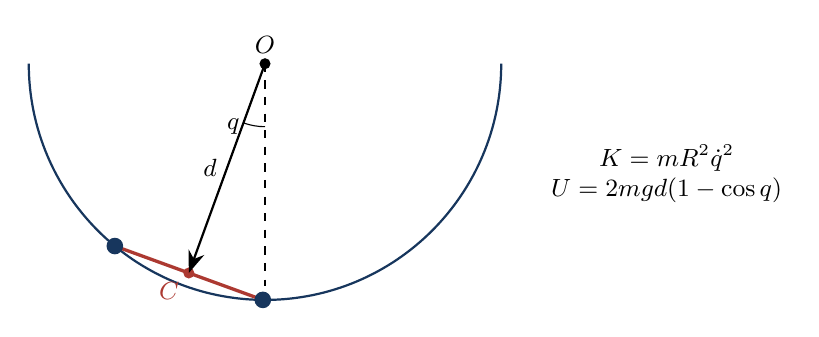
\begin{tikzpicture}

\draw[blue,thick](-3,0)arc(180:360:3);\fill(0,0)circle(2pt)node[above]{$O$};\draw[dashed](0,0)--(0,-2.828);\draw[very thick,red](-1.90707,-2.31583)--(-.02769,-2.99987);\fill[blue](-1.90707,-2.31583)circle(3pt);\fill[blue](-.02769,-2.99987)circle(3pt);\fill[red](-.96738,-2.65785)circle(2pt)node[below left]{$C$};\draw[arrow](0,0)--(-.96738,-2.65785)node[midway,left]{$d$};\draw(0,-.8)arc(-90:-110:.8);\node[left]at(-.2,-.8){$q$};\node[align=center]at(5.1,-1.4){$K=mR^2\dot q^2$\\$U=2mgd(1-\cos q)$};

\end{tikzpicture}
\begin{tikzpicture}

\draw[thick,blue](-2.8,0)arc(180:360:2.8);\draw[arrow](-3.3,0)--(3.4,0)node[right]{$y$};\draw[arrow](0,-3.2)--(0,.6)node[above]{$z$};\draw[dashed](0,0)--(0,-2.8);\draw[arrow](0,0)--(1.4,-2.425)node[midway,right]{$d$};\fill[red](1.4,-2.425)circle(4pt)node[right]{两截面投影重合};\draw(0,-.9)arc(-90:-60:.9);\node[right]at(.3,-.8){$\psi$};\node[align=center]at(-3.4,-2.4){$x=\pm l/2$\\杆方向不变};

\end{tikzpicture}
\begin{tikzpicture}

\node[box,fill=blue!8](a)at(0,0){中心$(X,Y)$\\二维等频振动};\node[box,fill=red!8](b)at(4.5,0){方位$\varphi$\\匀速转动};\node[box](c)at(2.2,-2){端点$\boldsymbol C\pm a\boldsymbol n$};\draw[arrow](a)--(c);\draw[arrow](b)--(c);\node[above]at(0,.65){$\omega=\sqrt{g/R}$};\node[above]at(4.5,.65){$\dot\varphi=v_0/l$};

\end{tikzpicture}
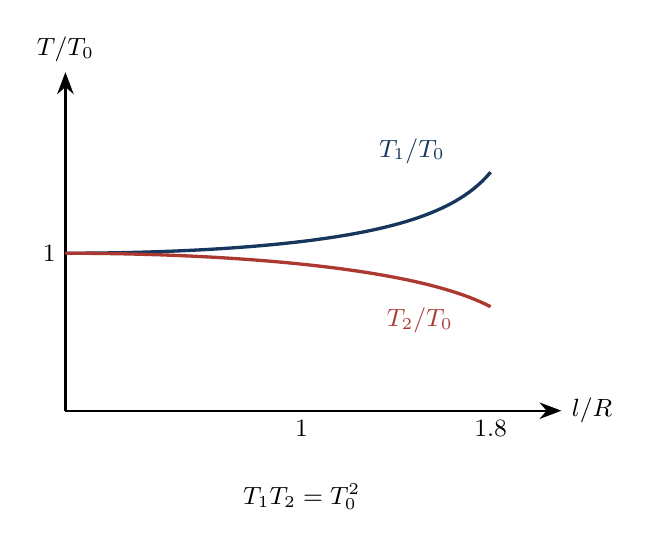
\begin{tikzpicture}
\draw[arrow](0,0)--(6.3,0)node[right]{$l/R$};\draw[arrow](0,0)--(0,4.3)node[above]{$T/T_0$};\draw[very thick,blue] plot coordinates {(0.00000,2.00000) (0.05455,2.00004) (0.10909,2.00017) (0.16364,2.00037) (0.21818,2.00066) (0.27273,2.00103) (0.32727,2.00149) (0.38182,2.00203) (0.43636,2.00265) (0.49091,2.00336) (0.54545,2.00415) (0.60000,2.00503) (0.65455,2.00600) (0.70909,2.00705) (0.76364,2.00818) (0.81818,2.00941) (0.87273,2.01072) (0.92727,2.01212) (0.98182,2.01362) (1.03636,2.01520) (1.09091,2.01688) (1.14545,2.01865) (1.20000,2.02052) (1.25455,2.02248) (1.30909,2.02454) (1.36364,2.02669) (1.41818,2.02895) (1.47273,2.03131) (1.52727,2.03378) (1.58182,2.03635) (1.63636,2.03902) (1.69091,2.04181) (1.74545,2.04470) (1.80000,2.04772) (1.85455,2.05084) (1.90909,2.05409) (1.96364,2.05745) (2.01818,2.06094) (2.07273,2.06456) (2.12727,2.06831) (2.18182,2.07219) (2.23636,2.07620) (2.29091,2.08036) (2.34545,2.08466) (2.40000,2.08910) (2.45455,2.09370) (2.50909,2.09846) (2.56364,2.10337) (2.61818,2.10845) (2.67273,2.11371) (2.72727,2.11913) (2.78182,2.12475) (2.83636,2.13054) (2.89091,2.13654) (2.94545,2.14273) (3.00000,2.14914) (3.05455,2.15576) (3.10909,2.16261) (3.16364,2.16969) (3.21818,2.17702) (3.27273,2.18460) (3.32727,2.19244) (3.38182,2.20056) (3.43636,2.20897) (3.49091,2.21768) (3.54545,2.22671) (3.60000,2.23607) (3.65455,2.24577) (3.70909,2.25584) (3.76364,2.26630) (3.81818,2.27716) (3.87273,2.28845) (3.92727,2.30018) (3.98182,2.31240) (4.03636,2.32512) (4.09091,2.33839) (4.14545,2.35222) (4.20000,2.36667) (4.25455,2.38177) (4.30909,2.39757) (4.36364,2.41411) (4.41818,2.43147) (4.47273,2.44969) (4.52727,2.46886) (4.58182,2.48904) (4.63636,2.51034) (4.69091,2.53285) (4.74545,2.55669) (4.80000,2.58199) (4.85455,2.60890) (4.90909,2.63761) (4.96364,2.66833) (5.01818,2.70128) (5.07273,2.73678) (5.12727,2.77516) (5.18182,2.81686) (5.23636,2.86238) (5.29091,2.91238) (5.34545,2.96767) (5.40000,3.02930)};\draw[very thick,red] plot coordinates {(0.00000,2.00000) (0.05455,1.99996) (0.10909,1.99983) (0.16364,1.99963) (0.21818,1.99934) (0.27273,1.99897) (0.32727,1.99851) (0.38182,1.99797) (0.43636,1.99735) (0.49091,1.99664) (0.54545,1.99585) (0.60000,1.99498) (0.65455,1.99402) (0.70909,1.99298) (0.76364,1.99185) (0.81818,1.99064) (0.87273,1.98934) (0.92727,1.98795) (0.98182,1.98647) (1.03636,1.98491) (1.09091,1.98326) (1.14545,1.98152) (1.20000,1.97969) (1.25455,1.97777) (1.30909,1.97576) (1.36364,1.97366) (1.41818,1.97146) (1.47273,1.96917) (1.52727,1.96679) (1.58182,1.96430) (1.63636,1.96173) (1.69091,1.95905) (1.74545,1.95627) (1.80000,1.95340) (1.85455,1.95042) (1.90909,1.94734) (1.96364,1.94415) (2.01818,1.94086) (2.07273,1.93746) (2.12727,1.93395) (2.18182,1.93033) (2.23636,1.92659) (2.29091,1.92275) (2.34545,1.91878) (2.40000,1.91470) (2.45455,1.91049) (2.50909,1.90616) (2.56364,1.90171) (2.61818,1.89712) (2.67273,1.89241) (2.72727,1.88756) (2.78182,1.88258) (2.83636,1.87745) (2.89091,1.87219) (2.94545,1.86677) (3.00000,1.86121) (3.05455,1.85549) (3.10909,1.84962) (3.16364,1.84358) (3.21818,1.83738) (3.27273,1.83100) (3.32727,1.82445) (3.38182,1.81772) (3.43636,1.81080) (3.49091,1.80368) (3.54545,1.79637) (3.60000,1.78885) (3.65455,1.78112) (3.70909,1.77317) (3.76364,1.76499) (3.81818,1.75658) (3.87273,1.74791) (3.92727,1.73899) (3.98182,1.72980) (4.03636,1.72034) (4.09091,1.71058) (4.14545,1.70052) (4.20000,1.69014) (4.25455,1.67942) (4.30909,1.66836) (4.36364,1.65692) (4.41818,1.64510) (4.47273,1.63286) (4.52727,1.62018) (4.58182,1.60704) (4.63636,1.59341) (4.69091,1.57925) (4.74545,1.56452) (4.80000,1.54919) (4.85455,1.53321) (4.90909,1.51652) (4.96364,1.49907) (5.01818,1.48078) (5.07273,1.46157) (5.12727,1.44136) (5.18182,1.42002) (5.23636,1.39744) (5.29091,1.37345) (5.34545,1.34786) (5.40000,1.32044)};\node[blue]at(4.4,3.3){$T_1/T_0$};\node[red]at(4.5,1.15){$T_2/T_0$};\node[left]at(0,2){1};\node[below]at(3,0){1};\node[below]at(5.4,0){1.8};\node[below]at(3,-.8){$T_1T_2=T_0^2$};
\end{tikzpicture}
\end{document}
